\documentclass[fleqn,10pt]{wlscirep}
\usepackage{multirow, subcaption, amsmath}

\DeclareMathOperator*{\argmaxA}{arg\,max}

\title{Teaching Machines to Process MEG Recorded Speech Tasks}
%\title{Comparing Machine Learning Techniques in Predicting Children's Age with MEG Recorded Speech Tasks}

\author[1,*]{Alice Author}
\author[2]{Bob Author}
\author[1,2,+]{Christine Author}
\author[2,+]{Derek Author}
\affil[1]{Affiliation, department, city, postcode, country}
\affil[2]{Affiliation, department, city, postcode, country}

\affil[*]{corresponding.author@email.example}

\affil[+]{these authors contributed equally to this work}

% Needs to be <=200 words.

\begin{abstract}
As language ability develops in children, the cortical structures employed in the brain progressively lateralize into typically the left hemisphere. Verb generation tasks have consistently demonstrated this phenomenon in both fMRI and MEG studies. With the recent increase in popularity of machine learning and deep neural networks (DNN)s, we consider whether a DNN trained with raw MEG signals can be used to predict the age of children performing a verb-generation task, a monosyllable speech-elicitation task, and a multi-syllabic speech-elicitation task. Previous work has explored taking DNNs designed for image processing and using them to process and classify encephalographic data with some success, but these architectures do little to acknowledge the structure of these data. Simple neural networks have been used extensively to classify data once broken down into features, but this requires extensive feature engineering and pre-processing. We present novel DNNs that can be trained from raw EEG/MEG data and mimic the feature-engineering pipeline. We demonstrate criteria the network use to make classification choices including relative weighting of channel measurements and preferred spectro-temporal information of un-mixed channels. Our data feature 92 subjects aged 4-18 recorded using a 151 channel MEG helmet. Our proposed model scores over 97\% single-fold binary classification accuracy distinguishing between greater or less than 10 years of age, and can classify publicly available EEG with state-of-the-art accuracy.

\end{abstract}
\begin{document}

\flushbottom
\maketitle
% * <john.hammersley@gmail.com> 2015-02-09T12:07:31.197Z:
%
%  Click the title above to edit the author information and abstract
%
\thispagestyle{empty}

\section*{Introduction}

The development of speech from infancy to adulthood is a remarkable and uniquely human process. Language and speech in the adult brain spans a diverse set of regions and interconnections from brain stem to cerebral cortex \cite{GuentherBook, Tourville2011, Hillis}, but higher level language abilities are a typically left-hemisphere lateralized process for approximately 90\% of the general population, although this  can range from 70\% to 95\% in populations with distinct left and right handedness respectively \cite{GuentherBook, Kadis2011, Yu2014}. Children develop this lateralization over time and show more bi-lateral activity as an inverse function of age \cite{Kadis2011, Ressel2008}. A common experiment paradigm for demonstrating this is the verb-generation task, which requires a subject to produce a verb they feel conveys meaning related to a stimuli with which they have been provided (e.g. an image) \cite{Kadis2011}. Speech articulation divorced from language is much less lateralized in comparison to {\em higher level} language faculties irregardless of age \cite{GuentherBook}, and in terms of cortical systems, heavily engages the Rolandic cortex to integreate somatosensory and motor control representations to command the speech articulators \cite{GuentherBook}. Despite the fact that this process is less lateralized than higher level language function, non-word monosyllabic, and multisyllabic experiments still show some left-lateralization \cite{Ghosh2008a}. We consider a dataset made up of a combination of a verb-generation task, the monosyllabic utterance /{\em pah}/ and the multisyllable non-word /{\em pah tah kah}/ with overlapping sets of subjects recorded using magnetoencephalography (MEG), in an effort to demonstrate age-related language and speech development. We expect that models making age distinctions with these data will leverage the phenomenon of lateralization to make age distinctions.

Machine learning (ML), especially neural networks has seen a recent surge in popularity as the costs for training has become practical for more scientists \cite{LeCun2015}. ML has been used in brain computer interface (BCI) tasks that typically require a classifier mechanism to make some prediction, and a common merging of language and speech tasks with BCI applications is the prediction of silent speech (imagined or covert) \cite{Sereshkeh2017, Guimaraes2007, Zhao2015a}. A typical pipeline is consistently employed for silent speech with BCIs \cite{RezaeiTabar2016}. First, data are collected and pre-processed using a variety of techniques, such as cropping, trial averaging, normalization, band-pass filtering, and spatial transforms such as principle component analysis (PCA), independent component analysis (ICA) and common spatial patterns (CSP) \cite{Muller-Gerking1999}. The goal of the preprocessing stage is to overcome the low signal-to-noise ratios typical of these types of recordings which complicate training in ML. After these initial steps, features are calculated from these data, of which there are a plethora of successful options, most commonly including spectral characteristics in the canonical brain rhythm bands ($\delta$, $\theta$, $\alpha$, etc.) and summary statistics. Finally, these features and their associated class labels are used to train a classifier. Often, classifiers like support vector machines (SVMs) or logistic regression are used, as they provide convex optimizations that are guaranteed to converge, and are less computationally taxing compared to (large) neural networks. An advantage of this overall approach is that expert knowledge about the data can help circumvent relatively poor signal quality and encourage ML models to distinguish between classes using established signal correlates. However, this comes with potential \emph{bias} of expert knowledge, and the underlying assumptions it may reinforce. In contrast, deep ML models can achieve many of the stages of this pipeline intrinsically. Although these deep-learning architectures are arbitrarily flexible classifiers, when they are trained in an end-to-end fashion, their hierarchical structures can also perform signal-processing in early layers that may be informative when compared to more directed techniques.

Taking an end-to-end machine learning approach to classifying new, perhaps previously difficult, problems that are not just BCI focused may provide new insights into underlying phenomena and also expand the pool of tools available to make sense of the increasingly large data produced by modern non-invasive brain activity recording techniques. Towards this, we propose two new deep neural network architectures trained end-to-end to predict the age of the subjects in our dataset. Since our dataset is of MEG recorded speech tasks, the prediction target of age with this context serves as the method for the ML classifier to find evidence of the development of language itself, rather than age-related distinctions alone. We compare their performance versus 


\section*{Proposed neural network architectures}

\begin{figure}[t]
  \begin{minipage}{0.47\textwidth}
    \centering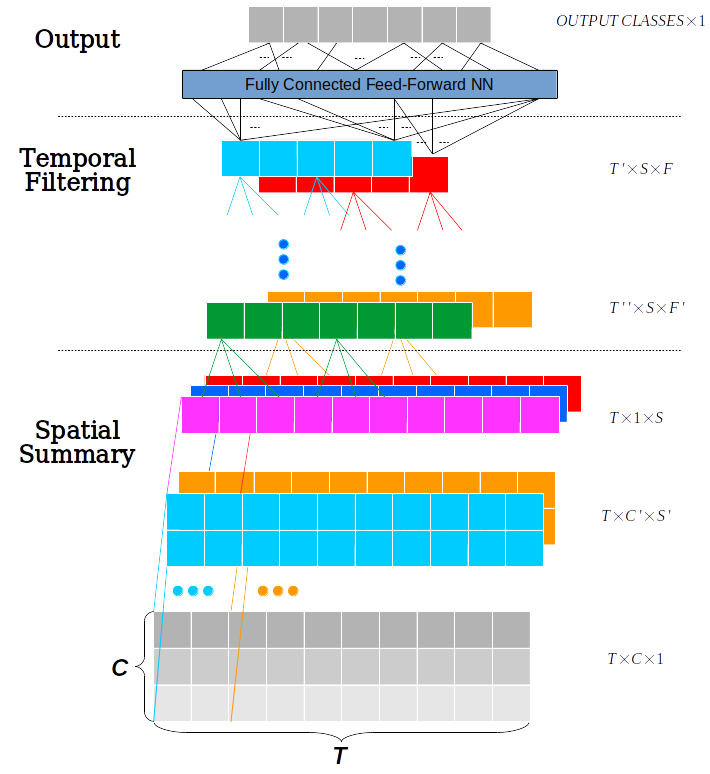
\includegraphics[width=\linewidth]{SCNN_architecture.png}
     \subcaption{This diagrams shows the Spatial summary convolutional network (which we refer to as SCNN). Processing flows from bottom to top, with the grey array representing a single trial. Each trial has $C$ channels and $T$ (where for our primary dataset: $C=151$ and $T=400$). The architecture is broken down into three stages, a {\em Spatial Summary} stage that performs convolutions exclusively across channels at each timepoint, thus not impacting the number of samples (the second dimension $T$ remains unchanged). Likewise, the {\em Temporal Filtering} stage performs convolutions exclusively across the time dimension. The output stage flattens the resulting output of the previous stages and uses a feed-forward network for final classification.}
  \end{minipage}
  \hspace*{\fill} % separation between the subfigures
  \begin{minipage}{0.47\textwidth}
    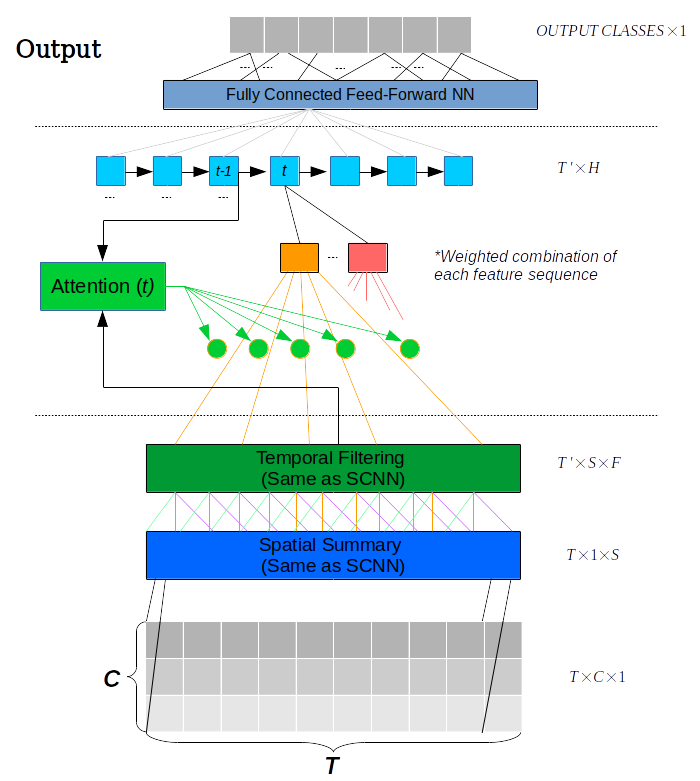
\includegraphics[width=\linewidth]{ALSTM_architecture.png}
     \subcaption{This diagrams shows the attention LSTM network. Processing flows from bottom to top, with the grey array representing a single trial. Each trial has $C$ channels and $T$ (where for our primary dataset: $C=151$ and $T=400$). This architecture extends the SCNN presented in \ref{fig:scnn_arch}, where the output of the {\em Temporal Filtering} stage in \ref{fig:scnn_arch} is fed as input to an LSTM enhanced with attention weighted input layer. Finally the output of the LSTM uses a feed-forward network for final classification.}
    %\label{fig:component_28}
  \end{minipage}
  \caption{}
  \label{fig:max_components}
\end{figure}

\subsection*{Spatial summary convolutional neural network (SCNN)} \label{sec:scnn}

The critical innovation of this architecture is to ensure spatial convolutions and temporal convolutions are performed separately. This results in a set of spatial filtering components that can be examined independently from temporal features. This also mimics the common feature approach pipeline of: spatial (channel) mixing, applying filter banks to mixed components to develop a set of features and then finally employing some classifier to use these features. In this architecture, the spatial convolutions ultimately span the length of the incoming channels, but rather than being a single linear layer we introduce non-linearity and multiple convolution layers that work together to construct a more flexible spatial filter, but one that still employs weight sharing at each step. We select a hyperparameter indicating the depth of the spatial filter, and then stack convolutional layers, where each layer reduces the spatial dimension until the final layer completely collapses it to a single dimension. After this, a number of temporal filters (i.e., convolutions over the temporal dimension) are applied to the new spatial mapping (the number is also a selected hyperparameter), and an optional average pooling layer to reduce the number of parameters and effectively low-pass filter these new features. Finally, the resulting features are flattened into a single vector and a fully connected neural network (FFNN) classifier is used as an output stage, with the number of layers determined again through hyperparameter search.

The first few layers of the CNN can be seen as a mapping from $R^{T \times C \times 1}$ to $R^{T \times 1 \times S}$ (the spatial filtering) to $R^{T' \times 1 \times F }$ (the temporal filtering) where $T' \leq T$, $C$ is the number of recording channels, $S$ is the number of spatial transformations, and $F$ is the number of temporal filters. In other words, a set $S$ of non-linear spatial transformations are applied to the $C$ channels, and then a set of $F$ temporal filters are applied to these new sequences.

Since the actual depth of spatial filtering and temporal filtering operations changes depending on the configuration selected by the hyperparameter search, consider an example architecture with two layers of spatial steps with $K_1, K_2$ kernels for each layer respectively. Let $\boldsymbol{X}$ be our input data with dimensions $T \times C$, where $T$ is the length of our temporal sequence and $C$ is the number of channels recorded. Also, as a result of the two spatial layers, we intend to produce the output $\boldsymbol{X}_{Spatial}$ with dimensions $T \times K_2$ where $K_2$ is the target number of {\em spatial components}. Starting with the first layer, and our $j'^{th}$ kernel $\boldsymbol{w}_{L_1}^j$, which has length $C'$, where $C' < C$, the output of filter $j$ of the first layer at time $t$ is then:

\begin{equation} \label{eq:scnn_s1}
  \boldsymbol{X'}_{t, i, j} = f\left(\sum_{k=0}^{C'} {\boldsymbol{w}_{L_1}^j}_k \boldsymbol{X}_{t,i+k}\right) \footnote{There are no bias terms needed here or later, as batch normalization \cite{Szegedy2015} renders them redundant and is employed throughout.}
\end{equation}

Where $\boldsymbol{X'}$ is a three dimensional tensor of shape $T \times (C-C') \times K_1$ and $f(x)$ is the neuron's non-linear function of choice. There is no integration of any temporal information besides $t$, and that for each kernel there are $C-C'$ sequences of length $T$, of which only the $i'{th}$ is shown above. Next, the second layer consists of kernel vectors $\boldsymbol{w}_{L_2}^s$ of length $C-C'$, which determine component $s$ of $K_2$ at time $t$ as follows:

\begin{equation} \label{eq:scnn_s2}
  {\boldsymbol{X}_{Spatial}}_{t, s} = f(\sum_{i=0}^{C-C'}{\boldsymbol{w}_{L_2}^s}_i \boldsymbol{X'}_{t, i, j})
\end{equation}

The temporal filtering operations behave like eq. \ref{eq:scnn_s1}, but each kernel in the temporal layer is applied across the {\em temporal} dimension of each kernel activation sequence of the previous layer.

\subsubsection*{Two-dimensional SCNN}

This architecture extends the SCNN above to data that are represented as 2D interpolated images of shape $D \times D$, rather than single dimensional sequences of channel values. In this architecture, rather than kernels being vectors, they are 2D square tensors that scale patches of the image. As such, eq. \ref{eq:scnn_s1} would instead be expressed:

\begin{equation} \label{eq:s2dcnn_s1}
  \boldsymbol{\hat{X}}_{t, m, n, j} = f(\sum_{m'=0}^{C''} \sum_{n'=0}^{C''} {\boldsymbol{w}_{L_1}^j}_{m', n'} \boldsymbol{X}_{t,m+m',n+n'})
\end{equation}

Which would result in a four-dimensional tensor $\boldsymbol{\hat{X}}$ with dimensions $T \times (C-C'') \times (C-C'') \times K_1$. Similarly modifying eq. \ref{eq:scnn_s1}, the same $X_{Spatial}$ is produced:

\begin{equation} \label{eq:scnn_s2}
  {\boldsymbol{X}_{Spatial}}_{t, s} = f(\sum_{m=0}^{D-C''}\sum_{n=0}^{D-C''}{\boldsymbol{w}_{L_2}^s}_{m,n} \boldsymbol{X'}_{t, m, n, s})
\end{equation}

\subsection*{Attention LSTM}

This is an extension of the SCNN, that uses an LSTM and attention mechanism after the spatial and temporal steps to provide the network a stronger ability to focus on aspects of the signal. In our experiments, we employ an architecture that is very similar to the encoding stage employed in Zhu {\em et al.} for the purpose of image-directed question answering \cite{Zhu}. Those authors used a pre-trained CNN and an LSTM-based encoder that was fed attention weighted inputs. Their attention mechanism provides an average weighting of the different convolutional feature maps which are combined with one-hot encoded word vectors representing the words in the questions.

In contrast, our implementation does not use a pre-trained CNN, but trains convolutional layers at the same time as the rest of the model. The attention serves as a mechanism to closely consider parts of the sequence depending on the state of the LSTM. So the intent is that the LSTM develops some sort of sequential processing that does not need to progress temporally sample by sample, but is flexible to consider any combination of samples that may become appropriate. Functionally, the attention mechanism pre-processes the output of the spatial summary (described in \ref{sec:scnn}) and optionally (a hyperparameter) filtering over time. The pre-processing is an average weighting of the entire temporal sequence of each incoming feature, depending on a function of the current LSTM hidden state and the feature sequence itself. So the input to the LSTM of feature $i$ at some point in the sequence $t$ of $T'$ is:

\begin{equation}
  x_{t,i}^{In} = \sum_{t=0}^{T'} \alpha_{t,i} X_{t,i}^{SCNN}
\end{equation}

Where $\alpha$ is defined in eq. \ref{eq:attn_nrg}. We select whether to use the full LSTM output sequence, or exclusively the last state output as part of our hyperparameter search, and optionally have several fully connected layers before the prediction layer.

\section*{Results}

\subsection*{Age classification}

\subsubsection*{Fine-grained prediction}

\begin{table}[htp]
  \caption{Classification accuracy mean and standard deviation across the seven age classes (lower inclusive, higher exclusive): 4-6, 6-8, 8-10, 10-12, 12-14, 14-16, $>$16. Also includes within-one (W1) accuracy mean and standard deviation. Strict accuracy has both feature and end-to-end approaches performing relatively well, but considering the within-one metric the un-augmented and temporal augmentation appear to perform consistently well. Friedman tests of within-one metric rejects the null-hypothesis of all equivalent performances and post-hoc analysis shows the SCNN model trained with the temporally augmented MEG data significantly outperforms the spatially augmented data SCNN and the SCNN trained with Audio data.}
  \makebox[\textwidth]{
  \centering
  \begin{tabular}{l l| c | c | c | c}
    \toprule
    \textbf{Dataset} & \textbf{Model} & \textbf{Mean \%} & \textbf{Dev. \%} & \textbf{W1 Mean \%} & \textbf{W1 Dev. \%}\\
    \toprule
    \multirow{5}{*}{Audio (feature)}
                     & Logistic Reg.       & 17.5 & 4.42  & 48.1 & 4.41 \\
                     & Linear SVM          & 17.2 & 5.15  & 54.4 & 1.91 \\
                     & FFNN                & 18.9 & 6.00  & 49.7 & 11.9 \\
                     & LSTM+A              & 23.8 & 7.08  & 58.4 & 6.33 \\
                     & SCNN                & 15.6 & 4.00  & 40.2 & 8.59 \\
    
    \midrule
    \multirow{5}{*}{MEG (feature)}
                     & Logistic Reg.        & 27.9 & 2.52  & 49.0 & 9.96 \\
                     & Linear SVM          & 28.5 & 0.79  & 53.0 & 2.82 \\
                     & FFNN                & 28.1 & 5.91  & 51.7 & 8.37 \\
                     & LSTM+A              & 20.7 & 6.90  & 50.1 & 11.6 \\
                     & SCNN                & 22.4 & 4.96  & 53.0 & 3.68 \\
    \midrule
    \multirow{2}{*}{MEG}
                         & LSTM+A              & 28.1 & 5.00 & 60.0 & 9.11 \\ 
                         & SCNN                & 28.6 & 7.91 & 59.9 & 11.0 \\
    \midrule
    \multirow{2}{*}{MEG (+crop aug.)}
                         & LSTM+A              & 26.3 & 2.07 & 50.2 & 2.36 \\ 
                         & SCNN                & 32.4 & 10.9 & 62.6 & 9.29 \\
    \midrule
    \multirow{1}{*}{MEG (+projection aug.)}
                         & SCNN                & 21.9 & 2.20 & 44.0 & 5.10 \\
    \midrule
    \multirow{1}{*}{MEG (proj.+noise aug.)}
                         & SCNN                & 15.0 & 5.10 & 37.4 & 9.83 \\
    \bottomrule
  \end{tabular}}
%  \caption{Classification accuracy mean and standard deviation across the seven age classes (lower inclusive, higher exclusive): 4-6, 6-8, 8-10, 10-12, 12-14, 14-16, $>$16. Also includes within-one (W1) accuracy mean and standard deviation. Strict accuracy has both feature and end-to-end approaches performing relatively well, but considering the within-one metric the un-augmented and temporal augmentation appear to perform consistently well. Friedman tests of within-one metric rejects the null-hypothesis of all equivalent performances and post-hoc analysis shows the SCNN model trained with the temporally augmented MEG data significantly outperforms the spatially augmented data SCNN and the SCNN trained with Audio data.}
  \label{tab:seven_way_results}
\end{table}

The results for models trained across the seven age classes are presented in table \ref{tab:seven_way_results}. Considering the strict accuracy metric alone, there is little differentiation between end-to-end and feature approaches. Both vary in mean scores in the 20-30\% range. The audio dataset, and the spatial projection with augmentation perform somewhat more poorly in this metric than the rest of the datasets and models. The SCNN with cropping augmentation appears to be the most successful model (considering highest mean accuracy), and this holds for the within-one metric as well. However it has quite a large variation and many models score similarly enough for this to mostly be coincidence. Interestingly when considering the within-one metric (W1 in table \ref{tab:seven_way_results}, the models trained with the audio dataset are in fact much more successful and in the case of the SVM perhaps dramatically so when compared to their strict accuracy. This indicates that some sort of pattern is being developed by the model, but is not powerful enough to distinguish among seven classes. The projection and projection+noise augmentation dataset perform quite poorly under both metrics, and additionally required much more training time and had many more parameters, and we would not recommend their use going forward without some change in number of training points or architecture configurations.

Examining the significance of the within-one metric scores using a Friedman test, we can reject that all the scores are equivalent with $\chi^2_{15}=36.494$ $p<0.0015$. Post-hoc Nemenyi analysis shows two significant ($p<0.05$ after single step correction) pairwise comparisons. In both cases the SCNN trained with the cropping augmented raw data significantly outperforms the SCNN trained with the audio dataset and the projection + noise datasets. This adds to an important observation that the models that are intended to be trained with end-to-end data are not {\em aided} by first extracting features, and with the audio dataset and SCNN clearly are {\em disadvantaged} by first extracting features. 

\subsubsection*{Binary classification}

\begin{table}[htp]
  \caption{Classification accuracy when constrained to the binary classification problem of $age >= 10$ versus $age < 10$.}
  \centering
  \begin{tabular}{l l | c | c}
    \toprule
    \textbf{Feature set} & \textbf{Model} & \textbf{Mean \%} & \textbf{Dev. \%} \\
    \toprule
    \multirow{5}{*}{Audio}
                         & Logistic Regression    & 54.3 & 6.44  \\
                         & Linear SVM             & 73.9 & 3.45  \\
                         & FFNN                   & 71.7 & 2.44  \\
                         & LSTM + Attention       & 67.5 & 13.9  \\
                         & SCNN                   & 65.9 & 9.35  \\
    \midrule
    \multirow{5}{*}{MEG reduced}
                         & Logistic Regression    & 63.5 & 5.64  \\
                         & Linear SVM             & 69.2 & 5.74  \\
                         & FFNN                   & 66.3 & 4.93  \\
                         & LSTM + Attention       & 72.3 & 1.74  \\
                         & SCNN                   & 69.7 & 7.03  \\
    
    \midrule
    \multirow{2}{*}{Raw Data}
                         & LSTM + Attention    & 92.6 & 5.79  \\ 
                         & SCNN                & 95.1 & 2.31  \\
    \midrule
    \multirow{2}{*}{Temporal Augmentation}
                         & LSTM + Attention    & 93.4 & 0.93  \\ 
                         & SCNN                & 89.2 & 7.93  \\
    
    \bottomrule
  \end{tabular}
%  \caption{Classification accuracy when constrained to the binary classification problem of $age >= 10$ versus $age < 10$.}
  \label{tab:binary_results}
\end{table}

Looking through table \ref{tab:binary_results} we notice what appears to be a very convincing difference in performance between feature-based and end-to-end approaches. The end-to-end approaches all score nearly 90\% or higher accuracy regardless of model used and interestingly, the combination of LSTM + attention model with temporal augmentation appears both highly accurate and consistent. When considering a single fold of the un-augmented raw data and the SCNN model, the accuracy is in fact over 97\%. Analysis with a Friedman test very distinctly shows real performance, with $\chi^2_{13}=52.789$ and $p<10^{-6}$. Despite these promising examinations, post-hoc analysis does not show that the end-to-end models unianimously outperform the feature engineered sets. All end-to-end models do significantly ($p<0.05$ after single-step correction) outperform logistic regression trained with either the audio or reduced MEG feature datasets, and the SCNN trained with raw un-augmented data also significantly outperforms the FFNN trained with the reduced MEG features dataset. Although this is not a unanimous demonstration that the end-to-end models are superior, we see this as a fairly promising indication of performance. Of particular interest are the SCNN models trained without temporal augmentation and the LSTM + attention model with temporal augmentation.


\subsection*{Secondary dataset classification}

\begin{table}[t]
  \caption{Classification accuracy of SCNN and LSTM with attention models proposed in this work as compared to the convolutional neural network implementation of a filter bank common spatial pattern (FBCSP) classifier from \cite{Schirrmeister2017}.}
  \centering
  \begin{tabular}{l l | c | c}
    \toprule
    \textbf{Feature set} & \textbf{Model} & \textbf{Mean \%} & \textbf{Dev. \%} \\
    \toprule
    \multirow{3}{*}{No Augmentation}
                         & FBCSP-CNN           & 70.9 & 12.6  \\
                         & SCNN                & 72.6 & 10.7  \\
                         & LSTM + Attention    & 73.3 & 13.6  \\ 
    \midrule
    \multirow{3}{*}{Temporal Augmentation}
                         & FBCSP-CNN           & 65.6 & 12.2  \\
                         & SCNN                & 35.1 & 14.2  \\
                         & LSTM + Attention    & 66.6 & 17.1  \\ 
    \bottomrule
  \end{tabular}
%  \caption{Classification accuracy of SCNN and LSTM with attention models proposed in this work as compared to the convolutional neural network implementation of a filter bank common spatial pattern (FBCSP) classifier from \cite{Schirrmeister2017}.}
  \label{tab:sec_results}
\end{table}

The results in table \ref{tab:sec_results} are meant as a verification that SCNN and LSTM + attention models are more generally applicable to MEG/EEG data and achieve results that are reasonably comparable to state-of-the-art end-to-end machine learning approaches. At first glance there are some increases in classification accuracy, but these are minor with respect to the deviation in performance (which is exceptionally large). Surprisingly, the augmented SCNN model performs extremely poorly with the augmented dataset. Although there appeared to be some drop in its performance against its un-augmented and LSTM + attention counterparts in the binary classification task of the primary dataset, it does not perform remarkably poorly as it does here. In this regard it performs relatively well in the seven-way classification task (and in fact has the highest mean accuracy). After performing paired Wilcoxon signed-rank tests of both SCNN and LSTM + attention models (excluding the dramatic outlier) with respect to the un-augmented CNN as FBCSP implementation, there were no statistically significant comparisons. It appears that these models are at least as good as a comparable state-of-the-art implementation.

\subsection*{Model Analysis}

We calculated the maximal activations as described in \ref{sec:max_act} for the model with the highest single fold test accuracy in the binary classification task to minimize creating artificial data that had characteristics that were not pertinent to the task at hand. This resulted in using the SCNN model trained with the second fold of the raw MEG dataset. The full listing of activations is found in Appendix \ref{apdx:max_act} for brevity. Here we focus on components (figure \ref{fig:max_components}) and spectrograms (figure \ref{fig:max_spectrograms}) that demonstrate characteristics that are common among the artificial activations.

\begin{figure}[h!]
  \begin{minipage}{0.31\textwidth}
    \centering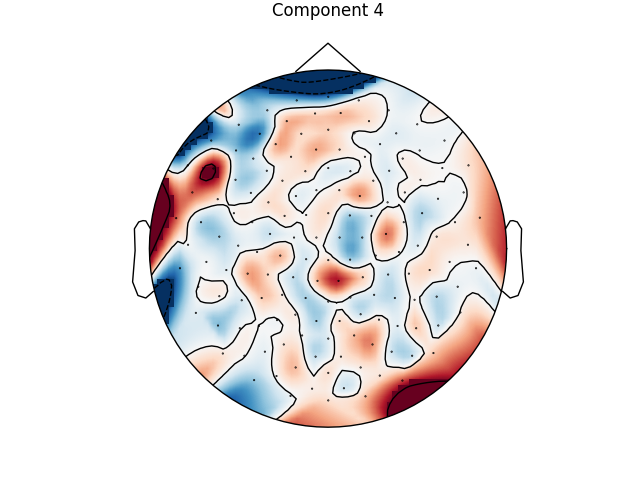
\includegraphics[width=\linewidth]{max_act/4.png}
     \subcaption{}
    \label{fig:component_4}
  \end{minipage}
  \hspace*{\fill} % separation between the subfigures
  \begin{minipage}{0.31\textwidth}
    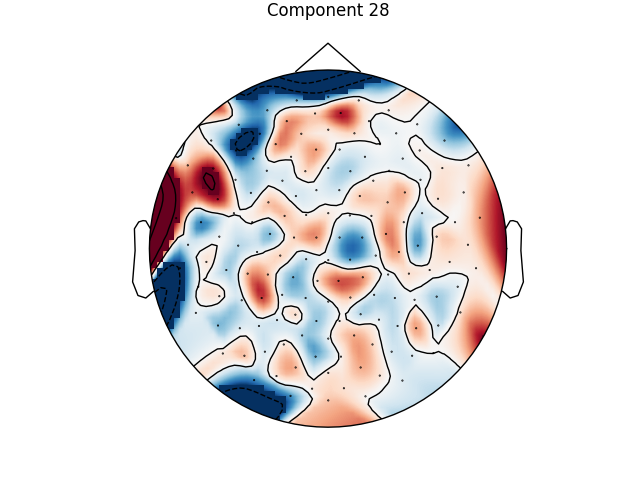
\includegraphics[width=\linewidth]{max_act/28.png}
     \subcaption{}
    \label{fig:component_28}
  \end{minipage}
   \hspace*{\fill} % separation between the subfigures
   \begin{minipage}{0.31\textwidth}
    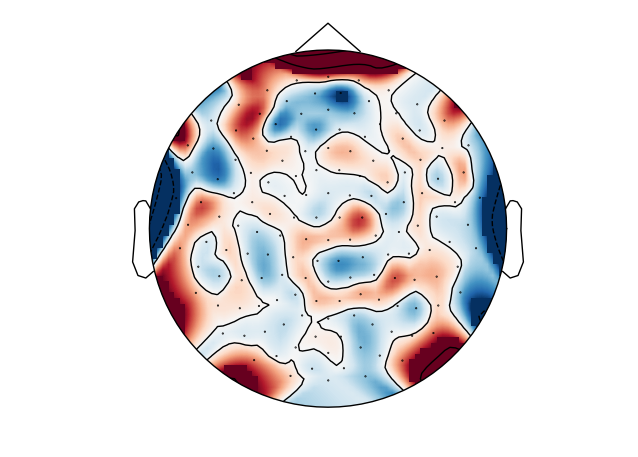
\includegraphics[width=\linewidth]{max_act/49.png}
    \subcaption{}
    \label{fig:component_49}
  \end{minipage}
  \caption[textfind]{Components (a) and (b) show a common pattern of spatial mixing, with a particularly strong weight localized around channels near the inferior frontal or perhaps dorsolateral prefrontal regions. This region is the only somewhat consistently strongly weighted region that is not exagerated by the edge effects of the interpolation. Component (c) shows a very nearly inverse set of weights compared to (a), in addition to what could be strong weights over the visual cortex (although edge effects of the interpolation make this hard to say). Components were plotted using the MNE python library. \footnotemark} \label{fig:max_components}
\end{figure}
\footnotetext{https://www.martinos.org/mne/stable/index.html}

\begin{figure}
  \begin{minipage}{0.24\textwidth}
    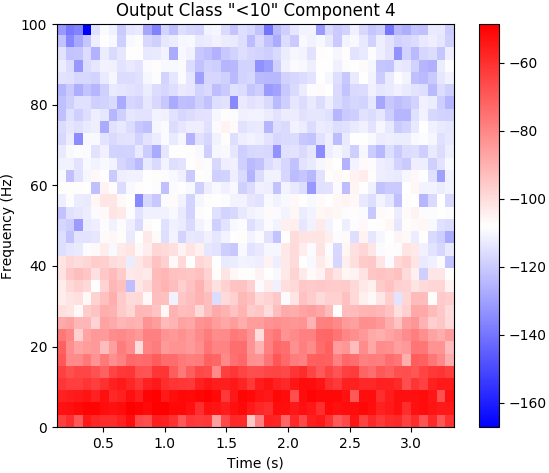
\includegraphics[width=\linewidth]{max_act/artificial_spec_4_0.png}
    \subcaption{}
%    \caption{} \label{fig:art_4_0}
  \end{minipage}
  \hspace*{\fill} 
  \begin{minipage}{0.24\textwidth}
    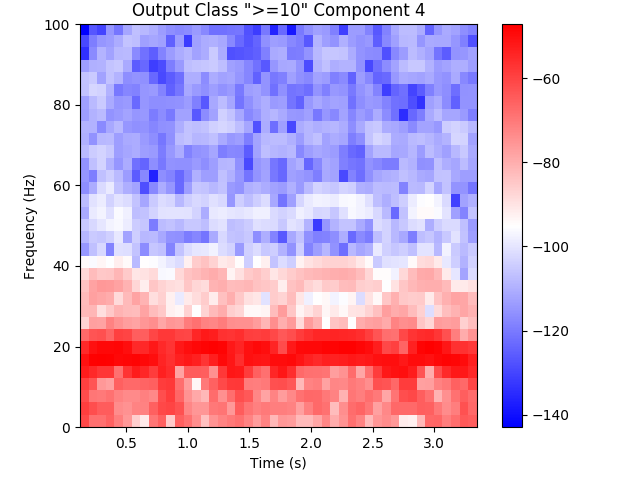
\includegraphics[width=\linewidth]{max_act/artificial_spec_4_1.png}
    \subcaption{}
%    \caption{} \label{fig:art_4_1}
  \end{minipage}
%  \vskip\baselineskip
  \begin{minipage}{0.24\textwidth}
    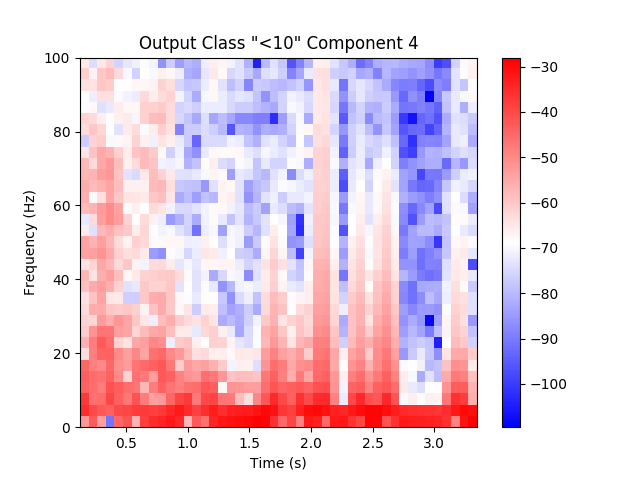
\includegraphics[width=\linewidth]{max_act/real_0_4.png}
    \subcaption{}
%    \caption{} \label{fig:real_4_0}
  \end{minipage}
  \hspace*{\fill} 
  \begin{minipage}{0.24\textwidth}
    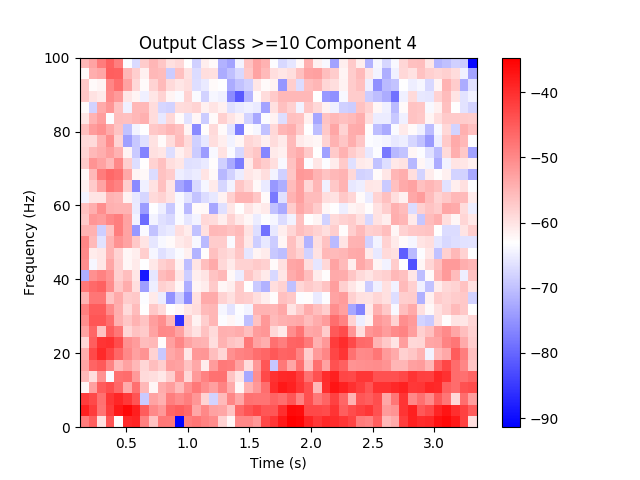
\includegraphics[width=\linewidth]{max_act/real_1_4.png}
    \subcaption{}
%    \caption{} \label{fig:real_4_1}
  \end{minipage}
  \vskip\baselineskip
  \begin{minipage}{0.24\textwidth}
    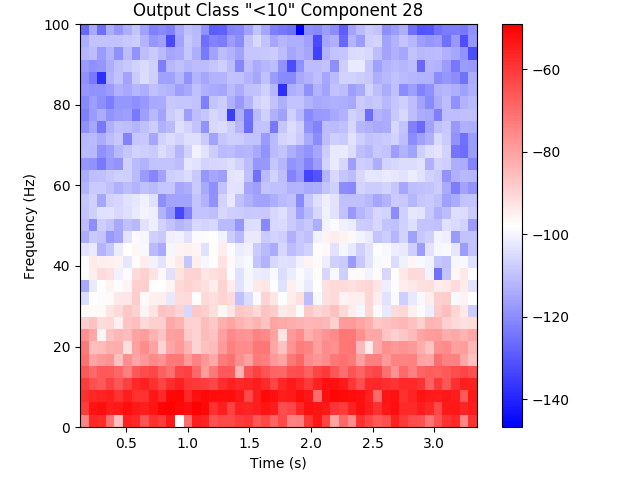
\includegraphics[width=\linewidth]{max_act/artificial_spec_28_0.png}
    \subcaption{}
%    \caption{} \label{fig:art_28_0}
  \end{minipage}
  \hspace*{\fill} 
  \begin{minipage}{0.24\textwidth}
    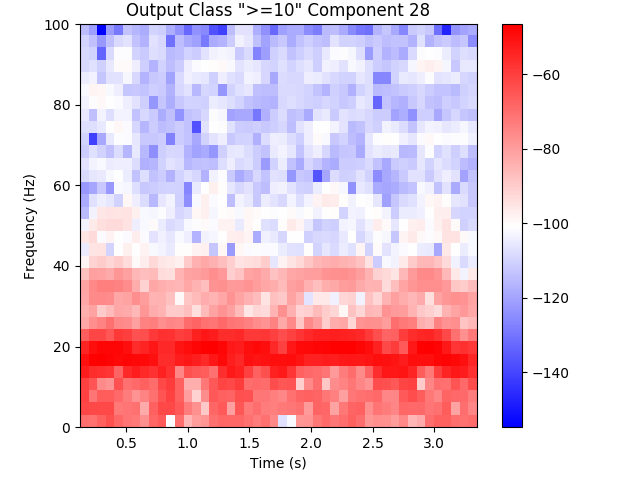
\includegraphics[width=\linewidth]{max_act/artificial_spec_28_1.png}
    \subcaption{}
%    \caption{} \label{fig:art_28_1}
  \end{minipage}
%  \vskip\baselineskip
  \begin{minipage}{0.24\textwidth}
    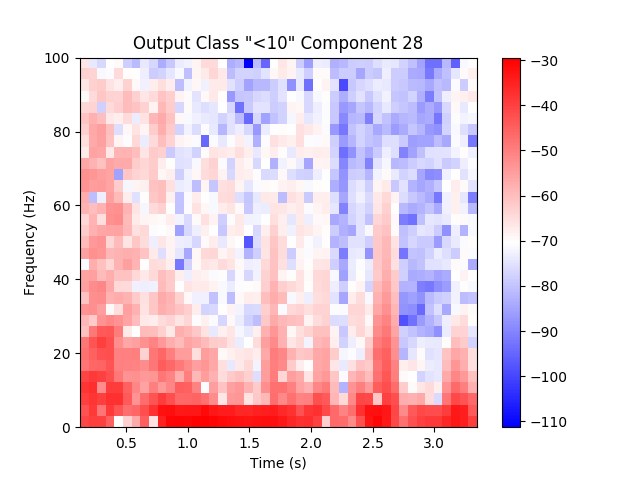
\includegraphics[width=\linewidth]{max_act/real_0_28.png}
    \subcaption{}
%    \caption{} \label{fig:real_28_0}
  \end{minipage}
  \hspace*{\fill} 
  \begin{minipage}{0.24\textwidth}
    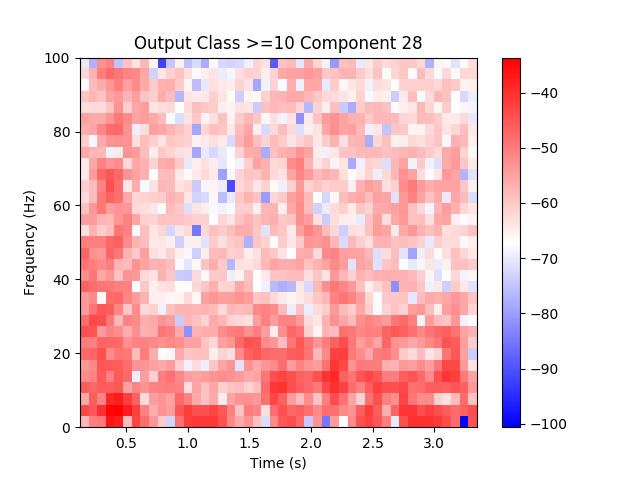
\includegraphics[width=\linewidth]{max_act/real_1_28.png}
    \subcaption{}
%    \caption{} \label{fig:real_28_1}
  \end{minipage}
  \vskip\baselineskip
  \begin{minipage}{0.24\textwidth}
    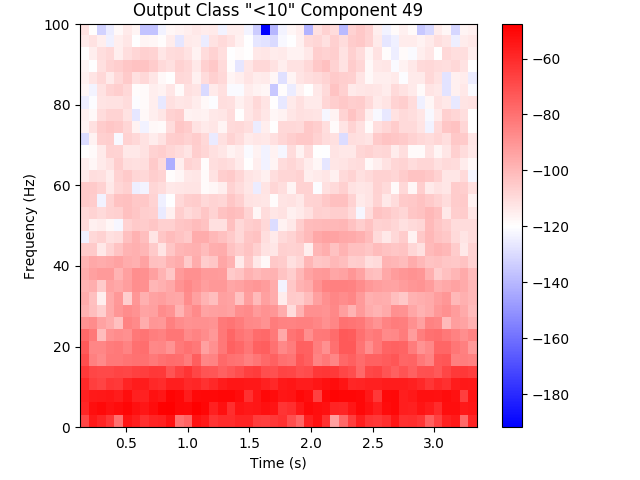
\includegraphics[width=\linewidth]{max_act/artificial_spec_49_0.png}
    \subcaption{}
%    \caption{} \label{fig:art_49_0}
  \end{minipage}
  \hspace*{\fill} 
  \begin{minipage}{0.24\textwidth}
    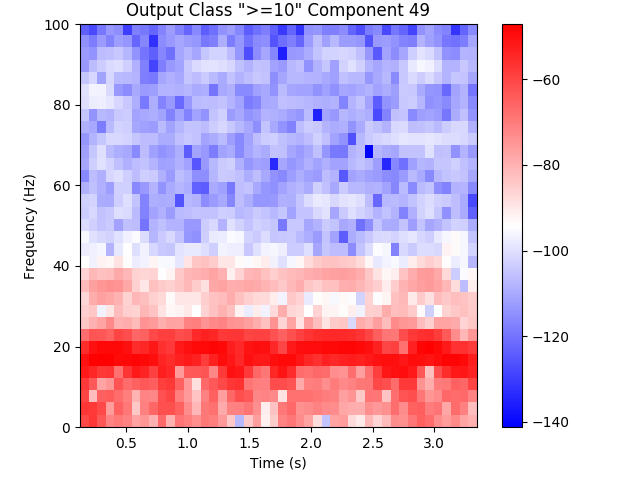
\includegraphics[width=\linewidth]{max_act/artificial_spec_49_1.png}
    \subcaption{}
%    \caption{} \label{fig:art_49_1}
  \end{minipage}
%  \vskip\baselineskip
  \begin{minipage}{0.24\textwidth}
    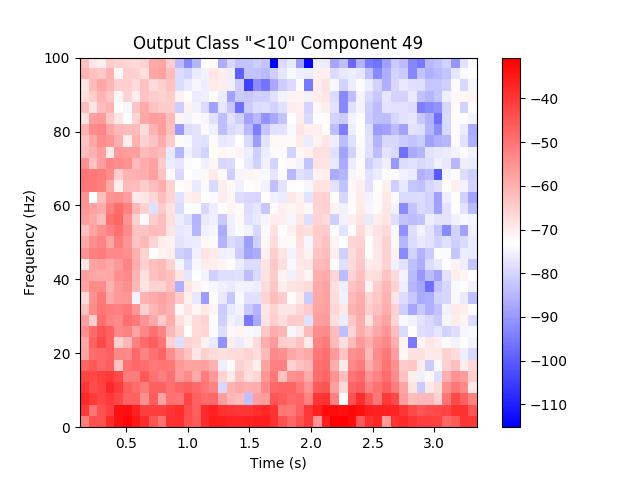
\includegraphics[width=\linewidth]{max_act/real_0_49.png}
    \subcaption{}
%    \caption{} \label{fig:real_49_0}
  \end{minipage}
  \hspace*{\fill} 
  \begin{minipage}{0.24\textwidth}
    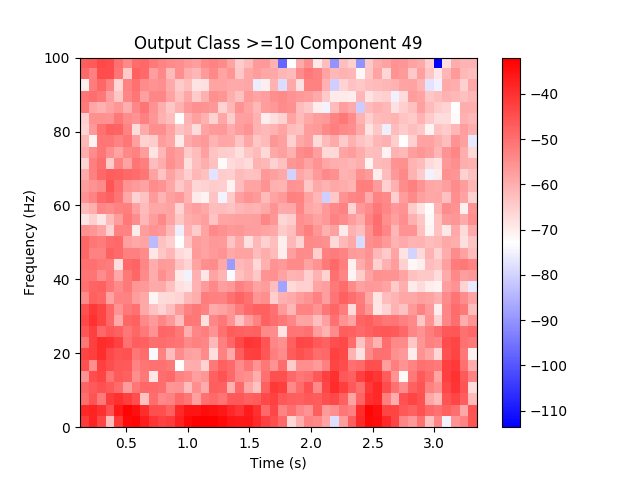
\includegraphics[width=\linewidth]{max_act/real_1_49.png}
    \subcaption{}
%    \caption{} \label{fig:real_49_1}
  \end{minipage}
  \caption{Plots \textbf{(a), (b), (e), (f), (i), and (j)} above represent artificially generated data that maximally activate the classes $<10$ and $>=10$ years old with respect to component 4 (figure \ref{fig:component_4}), component 28 (figure \ref{fig:component_28}) and component 49 (figure \ref{fig:component_49}). Where each row of spectrograms down corresponds to components 4, 28 and 49 respectively. Plots \textbf{(c), (d), (g), (h), (k), and (l)} show the two real datapoints that most significantly maximized the two classes for the same component.} \label{fig:max_spectrograms}
\end{figure}

Throughout the learned components, there is a common patch of strong weights found where what looks like the inferior frontal or perhaps dorsolateral prefrontal regions. All three components shown in figure \ref{fig:max_components} demonstrate this to some degree (although (c) has inverse sign). The artificially generated datapoints show fairly uniform spectrograms across all components, with spectral density concentrated between approximately $0-15$ H{\em z} in the $<10$ years old class, and concentration $15-22$ H$z$ for $>=10$ years old. All of the artificial datapoints are very stationary, and show no particular emphasis around the event time $t=1.5s$. The $>=10$ artificial data spectrograms do however show more activity overall in the high $beta$ low $gamma$ rhythms and this is particularly evident in components 4 and 49.

The real data, unlike the artificial data, unsurprisingly is not stationary, and does tend to show a marked change after the $t=1.5s$ mark. Again, much like the artificial data the profiles of each of the components were surprisingly homogeneous.

\section*{Discussion}

This work proposes two novel deep neural network architectures that can distinguish between children at different levels of speech development with at least equivalent if not greater accuracy than a feature based-pipeline. These networks also have the advantage of a consolidated training process (they are entirely trained through gradient-descent based optimization without intermediate steps) and also learn parameters that may have direct and interpretable connections to the task they are employed against. They also perform quite comparably against the state-of-the-art in a completely separate BCI task. 

Although some models succeed in classifying the examples in the primary dataset, many (reasonable) models during hyperparameter searches and initial investigations failed to perform better than random chance. This implies that the hyperparameter selection is of critical importance, and in many cases it will not suffice to try incompatible architectures with parameters that are just {\em good enough}. We see this as further indication that the application of deep-learning here needs continued development to establish a tool-set of appropriate architectures and stronger guiding principles for this type of data.

Towards determining if the /{\em pah}/ and /{\em pah tah kah}/ vocalization trials or the verb generation experiment trials had a greater impact on performance in the end-to-end learning, we trained the raw SCNN model using these datasets separately. Interestingly they seemed to have difficulty outperforming random chance on their own (although these were somewhat earlier model iterations). This suggests that despite being slightly different experiments perhaps at the very least the increase in training data is crucial to enabling the performance of these more powerful ML models.

When establishing the reduced set of MEG features, we evaluated the `optimal' reduced set of features against other subsets of the MEG features to determine if they were justifiably more powerful. First, we randomly extracted a subset of 172 features. Performing multilinear regression on this random selection of features remained insignificantly different than using all features. We also considered a set of the 172 most correlated MEG features among those with $p \geq 10^{-5}$, which accounts for high, but potentially quite variable, correlations. Surprisingly, this improves accuracy slightly on average over using all features, but with a much larger variance. The optimum solution remained to force $p<10^{-5}$ for the feature set we focused on. % These {\em ad hoc} analyses seem to suggest that increases in performance depend not on merely reducing dimensionality blindly, but on selecting {\em consistently} correlated features.

%Performing ICA separately for each stimulus results in different components, naturally. In other words, component $c_i$ with respect to the /{\em pah}/ data is different than component $c_i'$ with respect to the VG data. Future work should consider the sensitivity of any analysis to the stimulus, and be able to generalize ICA analyses that were performed on different data sets, particularly since our approach to end-to-end spatial mixing is done with no consideration for which stimuli were used at training time. Additionally, while we take the spatial patterns from the end-to-end models as similar in principle to ICA, unlike ICA there is no strong source separation premise underlying the neural network approach. In fact neural networks are notorious for developing redundant operations, and at times designers must take many steps to minimize this behaviour.

During hyperparameter search and initial investigations, we considered {\em label-smoothing} \cite{Pereyra2017} while training the seven-way classification task. This means rather than using {\em one-hot} encoded true labels for the seven classes, we created a discrete pseudo-normal distribution centred at the true label. In practice this meant setting the true label to $0.6$ and its neighbouring classes to $0.2$ (and at the upper and lower ends we set the true label to $0.8$ with its neighbour again $0.2$). This in effect created a distribution that the models were expected to learn, rather than discrete classes. We also considered L2 SVM output layers as described in \cite{Tang2013a}, but found that they performed no better than a softmax output layer and tended if anything to perform slightly worse overall. We also spent some time exploring CNN architectures that developed features using data across time and space, but found very little success with these methods, (these experiments were very preliminary and consisted of a few heuristic selections of parameters). Interestingly the failures were generally not the result of over-fitting, as they found fitting to the training data surprisingly difficult (they could however memorize smaller subsets of the data). On the other hand the spatial projection dataset was {\em particularly} susceptible to overfitting to the training data. We believe that the redundant data in this presentation made generalization {\em much} more difficult. Unless considering datasets with many more training points, or employing some more effective regularization techniques we would not recommend proceeding with spatially projected data in future work. 

A somewhat unconventional approach that we took was to train the early convolution layers in conjunction with the subsequent LSTM + attention layers. Previous work favours using pre-trained networks, but this is mostly due to the ubiquity of pre-trained image networks which make the need for re-training an image network unnecessary and time-consuming. We instead have the added challenge of training a subset of the network to calculate a range of spatial and temporal filters, and then learn how to weight the sequence of these features. Future work may benefit from seperating these tasks more to follow previous successes with attention mechanisms. For example the formulation of attention that we borrow from most \cite{Zhu}, is a transduction task that focuses on different aspects of a {\em pre-trained} CNN for image classification and then answers questions about the images using a LSTM+attention layer. This allows them to keep a relatively small training set (one that is less than one million examples) despite such a complex task. An interesting direction for future work might be to develop some general MEG/EEG applicable early layers out of the combination of many different open-access datasets, and then employ LSTMs with attention mechanisms for fine-tuning for a specific task.

Although no statistically significant conclusions can be made as to the power of the SCNN model versus its LSTM + attention counterpart, we should point out that when employing the cropping augmentation, particularly with the secondary dataset, and to a lesser extent the binary classification task, the SCNN performs poorly as compared to the LSTM+attention. This makes some intuitive sense, since the attention mechanism should allow for some insensitivity with respect to event offset, in a more powerful sense than the SCNN, which would rely on a later pooling layer for example to provide this functionality (and thus have a limited range). In practice however, the SCNN trained with cropping augmentation performed much better in the seven-way classification task than any other model.

As we mentioned in section \ref{sec:max_act}, previous successes with maximal activations such as in Yosinski {\em et al.} employ a heuristic combination of regularization methods that encourage the input data to behave according to patterns the data that will be provided to the network takes \cite{Yosinski2015}. An interesting example Yosinski {\em et al.} provide, is the use of Guassian blur penalization that penalizes the production of images with high spatial frequency \cite{Yosinski2015}. We notice that in fact in our work, the spectrograms we calculate in fact do demonstrate some surprisingly high frequency activity. It may be practical to not just begin with data that have $1/f$ spectral density as we do with our data, but to also penalize deviations from this expectation. There may be more that can be done to regularize artificial data and this warrants further study.

Future work that investigates maximal activations should also take steps to gauge event related synchrony/desynchrony in the context of artificial data, as the current consideration of spectrograms alone is fairly limited. Work in this direction may prove particularly interesting since convolution operations as employed in CNNs are in effect also calculating a correlation measure \cite{GravesRNNBook}.

These results are interesting as a demonstration of the ability of end-to-end models to predict language development, but neural networks show perhaps even greater promise as computational modelling techniques that to some degree mimic the human brain. For example \cite{cichy2016} compare the activations of a image classifier CNN and the MEG and fMRI activity of 15 subjects viewing the same test objects as the CNN. Interesting future work would be to employ new deep neural network architectures that predict speech output or articulator positions with the same data, and explore their connection to real brain structures and/or other speech models such as \cite{Guenther2005}.

\section*{Methods}

\subsection*{Primary dataset: Synchronized MEG and speech recordings}

\begin{table}[t]
  \centering
  \begin{tabular}{ l@{}c c c c }
    \toprule
    \textbf{Stimuli} & \textbf{Age range} & \textbf{Subjects} & \textbf{Trials}  & \textbf{M/F Split} \\
    \midrule
    /{\em pah}/~~~                    & $4.1-18.1$   &   $89$   &   $115$   &   $0.45/0.55$ \\
    /{\em pah tah kah}/~~~            & $4.1-18.1$   &   $83$   &   $115$   &   $0.45/0.55$ \\
    VG~~~                             & $5.7-18.0$   &   $28$   &   $81$    &   $0.42/0.58$  \\
    \bottomrule
  \end{tabular}
  \caption{Participant demographics, across stimuli type. The two tasks involve considerable participant overlap.}
  \label{tab:subjects}
\end{table}

These data were originally recorded to examine age- and sex-related developmental language differences in children by \cite{Doesburg2016} and \cite{Yu2014}. Table \ref{tab:subjects} summarizes participant demographics. Each participant spoke English as their first language and had no known or suspected histories of speech, language, hearing, or developmental disorders, according to their parents. Prior to the experiment, children received two standardized clinical tests: the Peabody Picture Vocabulary Test (PPVT) \cite{Dunn97} and the Expressive Vocabulary Test (EVT) \cite{EVT}. All children's scores were at or above expected scores for their ages on the PPVT and EVT, and their speech showed neither signs of articulatory difficulties nor any significant effect of age, as visualized in Figure \ref{fig:ppvtevt}. In total, 80 participants were right-handed, 5 were left-handed, and 7 were ambidextrous, according to the Edinburgh assessment \cite{Oldfield1971}, there is no significant variation of handedness with age.

Three distinct speech-elicitation stimuli were used. The first two were of the monosyllable /{\em pah}/ and the multisyllabic sequence /{\em pah tah kah}/, respectively. These were simple enough for young children and are part of the diadochokinetic rate (DDK) test, which can be used to evaluate neuromuscular control in motor speech disorders. Prior to acquisition, the experimenter demonstrated the productions of each stimuli, without word-like prosodic patterns. The third experiment was an overt verb generation (VG) task in English, where subjects were presented with an image with which they were familiar, and were asked to produce a verb associated with the object \cite{Doesburg2016}.

Recordings were made in a sound-proof room, with each participant lying supine in a magnetically shielded room in the Neuromagnetic Lab of the Hospital for Sick Children in Toronto, using a CTF whole-head MEG system (MEG International Services Ltd., Coquitlam, BC, Canada). The system recorded all 151 MEG channels, and a single audio channel, with a sampling rate of 4 kHz. We perform a bare-minimum cleanup of the data were we resample MEG signals at 200 Hz, and band-pass filter between 0.5 Hz and 100 Hz, to remove offsets and accommodate the canonical ranges of $\delta$, $\theta$, $\alpha$, $\beta$, and $\gamma$ activity. Electrooculography (EOG) artifacts are removed using second order blind identification (SOBI) automated blind source separation as provided by EEGlab \cite{Delorme04eeglab}.

Using these data, Doesburg {\em et al.} \cite{Doesburg2016} predicted language ability as an increase in network synchrony, particularly in the theta band with the increase of age during verb-generation (VG) tasks in children and adolescents. They observed a significant increase in the number of synchronous regions with older adolescents, compared with younger children. Yu {\em et al.} \cite{Yu2014} specifically focused on four regions of interest: inferior frontal regions, dorsolateral prefrontal regions, temporal-parietal regions, and superior temporal regions. They noticed distinct profiles of de-synchrony over time in VG tasks for children within five age ranges (i.e., 4-6, 7-9, 10-12, 13-15, and 16-18 years of age).

\subsection*{Supplementary dataset: BCI Competition IV, Dataset 2a}

In an effort to compare the potential success of our end-to-end models to previous work, we also trained some of our proposed models using the BCI Competition IV EEG Dataset \cite{Tangermann2012}. This dataset has featured in several other attempts to apply deep learning to neurophysiological data  and is freely available online \footnote{http://bnci-horizon-2020.eu/database/data-sets}.

These data consist of EEG recordings of 9 subjects performing 4 different imagined motor tasks: left hand, right hand, both feet, and tongue. These recordings were broken up into two separate sessions for each subject recorded on different days. Each of these sessions consisted of 6 sets of 48 trials separated by a short break, where the 48 trials were 12 executions of each of the 4 tasks. Thus a total of 288 trials were recorded per session. One session is considered training data, and the second is used as evaluation requiring some carry-over performance between days. The recordings consist of 22 EEG electrodes, and 3 monopolar EOG electrodes, all recorded at 250 Hz and bandpass filtered between 0.5 and 100 Hz. Additionally, a 50 Hz notch-filter was used to minimize line noise. The trials themselves are available as 6 second recordings, where the first two seconds consist of presenting each subject a fixation point. At 2s through 3.25s a task stimuli was presented to the subjects. There is additionally some EOG only trials per session that we discard. 

There are several challenges to using this dataset as a benchmark. It uses a different task entirely and contains EEG rather than MEG recordings, so there are far fewer EEG channels than the number of MEG channels from our primary dataset. The participants also come from a different population than the children and adolescents of our primary data. Regardless, we use this dataset to ensure that our model architectures have some sort of generalizability within this domain that can be compared against previous work. 

\subsection*{Supplementary dataset: BCI Competition IV, Dataset 2a}

In an effort to compare the potential success of our end-to-end models to previous work, we also trained some of our proposed models using the BCI Competition IV EEG Dataset \cite{Tangermann2012}. This dataset has featured in several other attempts to apply neural networks trained end-to-end to neurophysiological data \cite{Schirrmeister2017,Tabar2017,Lawhern2017,Sun} and is freely available online \footnote{http://bnci-horizon-2020.eu/database/data-sets}.

These data consist of EEG recordings of 9 subjects performing 4 different imagined motor tasks: left hand, right hand, both feet, and tongue. These recordings were broken up into two separate sessions for each subject recorded on different days. Each of these sessions consisted of 6 sets of 48 trials separated by a short break, where the 48 trials were 12 executions of each of the 4 tasks. Thus a total of 288 trials were recorded per session. One session is considered training data, and the second is used as evaluation requiring some carry-over performance between days. The recordings consist of 22 EEG electrodes, and 3 monopolar EOG electrodes, all recorded at 250 Hz and bandpass filtered between 0.5 and 100 Hz. Additionally, a 50 Hz notch-filter was used to minimize line noise. The trials themselves are available as 6 second recordings, where the first two seconds consist of presenting each subject a fixation point. At 2s through 3.25s a task stimuli was presented to the subjects. There is additionally some EOG only trials per session that we discard. 

% There are several challenges to using this dataset as a benchmark. It uses a different task entirely and contains EEG rather than MEG recordings, so there are far fewer EEG channels than the number of MEG channels from our primary dataset. The participants also come from a different population than the children and adolescents of our primary data. Regardless, we use this dataset to ensure that our model architectures have some sort of generalizability within this domain that can be compared against previous work.

\subsection*{Sensor projection}\label{sec:sens_proj}

To better represent the spatial structure of the recordings, we consider a series of image representations of the data. The data are originally represented as 2-dimensional arrays whose first dimension corresponds to samples in time, and the second dimension is of length 151, corresponding to the MEG channels in no spatially significant ordering. To represent the spatial nature of the data, the locations of the 151 channels of the MEG sensor array for each experiment are projected using an azimuthal projection (also known as polar projection) onto a two-dimensional grid sized $h \times v$. This transform preserves the distance between each point and a central reference point. The raw values of each sensor are then interpolated over the 2-dimensional image, where each pixel in the image is assigned the value of the nearest (projected) sensor. This generates a series of images, i.e. a three-dimensional datapoint with dimensions $samples \times  h \times v$ where $h$ and $v$ are hyperparameters that we search for before final training. A similar approach was used in Bashivan {\em et al.}, where EEG data were projected and then interpolated into a series of images but, instead of using raw data as we do here, they created multiple channels which represented different spectral features (in their case, the $\theta$, $\alpha$, and $\beta$ frequency bands) \cite{Bashivan2016}. We choose not to take this approach, as this would increase the dimensionality of the problem immensely and, as implemented by Bashivan {\em et al.} \cite{Bashivan2016}, the approach requires a strong assumption of how distinguishing data distributes across particular spectral bands and we intend for the network to distinguish such characteristics without prior knowledge.

\subsection*{Cropping}

To augment the number of training points available, the entire trial is split into multiple training examples by taking subsections of each trial that still include the event onset. Effectively, rather than one training datapoint for each trial, a sliding window smaller than the length of the trial is used to crop many points, where each point has the event onset localized in a different place. The premise behind this augmentation is that with the event localized in different places, an architecture like a convolutional or recurrent network can learn temporal filters that are agnostic of a specific onset time and thus should be more generalizable. Previous work that has taken a similar approach include Schirrmeister {\em et al.} \cite{Schirrmeister2017} and Sun {\em et al.} \cite{Sun}, but alternatively to our work, they assume a convolutional input stage and provide variable temporal length training points rather than fixed length crops. %We uniformly select a single crop position for each trial every epoch, rather than inflating the number of points in the dataset.

%% \subsubsection{Subsampling}

%% We take advantage of the high sampling rate of the recordings ($4kHz$) being used with respect to the frequency ranges that that we keep  for analysis and examine whether different sub-sampling of the data is a viable augmentation strategy. Filtering is still applied as before to minimize aliasing artifacts, and then we augment the number of samples by re-sampling at a frequency of $200 Hz$

\subsection*{Adding sensor noise}

To our knowledge, there are few examples of data augmentation with respect to the {\em location} of channels for training neural networks. Krell \& Kim, developed a rotational strategy of EEG data augmentation where they saw success in increasing classification accuracy for their particular processing chain using rotations in three-dimensional space of $\pm 18^{\circ}$ around the y- and z-axes \cite{Krell2017}. We consider an alternative augmentation strategy that we hypothesize may be more appropriate for MEG data, where the location of a sensor (after projection \ref{sec:sens_proj}) is subject to Gaussian distributed noise (truncated within a single deviation), with the recorded position being the mean of the distribution and variance being a hyperparameter to be selected. As MEG helmets tend to be slightly large for most people, and this effect is exagerated when considering small children such as in our primary dataset, this noisy sensor augmentation is a simple modeling of this source of error to enable better generalization with this higher dimensional data (sensor projection of course increases the dimensionality of the data significantly).

\subsection*{Model analysis and visualizations} \label{sec:max_act}

Explaining {\em what} a trained neural network has learned is an on-going area of research, and a particularly important one. For neural-network based models to be significantly useful beyond their successes as classifier tools, understanding what they are doing is crucial. There are currently two directions of work that address this, one in which (optionally modified) selections from datasets are fed into an already trained model and the sensitivity of specific layers or neurons are examined, and a second in which artificial data are developed by maximizing the outputs of a trained model with respect to artificial data (with no reliance on training points in particular) \cite{Yosinski2015}. We take the latter approach to develop artificial inputs that maximally activate key points in our models, which involves performing regularized gradient-ascent of an output $f_o(x)$ within the fully trained model with respect to the input $x$. So that we produce an artificial datapoint $x_{max}$ where:

\begin{equation} \label{eq:max_act}
  x_{max} = \argmaxA_x(f_o(x) - R(x))
\end{equation}

Here we summarize any regularization penalties as $R(x)$. \cite{Yosinski2015} show that crucial to the success of this technique is to ensure good prior distributions on the artificial data, so in this spirit we begin with randomly initialized data that have a spectral density that decreases with $1/f$ and zero mean, thus conforming to general encephalographic recordings. We also use L2 regularization on our data-points which helps prevent unbounded growth during the ascent which in effect prevents some strongly relevant features from eclipsings some features that are important but less impactful on the outputs. The iterative maximized input value is then:

\begin{equation} \label{eq:max_act_update}
  \hat{x}_{max} \leftarrow \eta \left(\hat{x}_{max} + \frac{\partial }{\partial x}(f_o(x) - \theta \cdot {}\sum_ix_i^2) \right)
\end{equation}

Where we heuristically select a step increase of $\eta = 0.2$ and L2 regularization of $\theta = 0.05$. We then iterate up to $10,000$ times, stopping if no progress is made for more than 5 steps. Additionally we normalize the derivative in eq. \ref{eq:max_act_update} for each step by its RMS value to make more stable (less oscillatory) progressions.

We construct maximal inputs for two sets of input-output pairs in the trained (using the primary dataset) end-to-end models. The first is between the model's normal input, and the end of the final-most spatial convolution layers, which we then interpolate across true channel locations for our MEG machine to demonstrate a rough localization of spatial components/mixing. The second input-output pair is between the input to the first temporal convolution (the output of the last spatial) and the final model output (classification stage). This is to generate data that highlight temporal features of the patterns of mixed sensors, which we do by calculating a spectrogram (Hann windows with 50 samples overlap and 64 FFT bins) for each component and output class.

\subsection*{Model training procedures} \label{sec:train_proc}

Each model is tested using 5-fold cross-validation against a held-out group of subjects. The test subjects are selected to have a similar distribution of the number of trials in each age range. The remaining subjects are ordered based on the number of trials they performed and their trials are distributed across the 5 folds in this order to create an approximately equal number of trials in each fold. The range in number of training points between folds was 3838 through 4078. We quantitatively evaluated the similarity between the 5 folds and test set using a K-sample Anderson-Darling test, where we found $A^2=-0.271$ with $p=0.61$. In the supplemental dataset, the training versus test datasets are separated in advance for intra-subject training.

We use Keras \footnote{https://keras.io/} with a Tensorflow \footnote{https://www.tensorflow.org/} backend to build all of the following models, and use either stochastic gradient descent or the Adam optimizer\cite{Kingma2015} when performing back-propagation updates. When training the neural networks, we select between three different activation functions: the rectified linear unit (ReLU) \cite{He2015a}, the exponential linear unit (ELU) \cite{Clevert}, and the scaled ELU (SELU) \cite{NIPS2017_6698}. All layers are batch-normalized \cite{Szegedy2015} after activation. We additionally employ L2-norm weight regularization for all trainable weights, excluding those of RNNs. We apply dropout \cite{Srivastava2014} after all fully-connected layers, and both max-pooling and spatial dropout \cite{Tompson2015} to all convolutional layers. These techniques are not necessarily applied to the FBCSP-like model from \cite{Schirrmeister2017}, which is reproduced by examining their source code.

All hyperparameter selection is done using Bayesian parameter optimization with Hyperopt \cite{Bergstra2013} including: learning rate, regularization penalty, dropout rates, number of adjacent activations to pool, number and layers of hidden units, receptive fields, and activation functions for all appropriate models. Hyperparameter searches are performed for 100 iterations. Appendix \ref{apdx:hyperparams} has a more detailed description of search spaces used and the specific values for parameters that were ultimately selected.

\bibliography{sci_reports}

\section*{Acknowledgements (not compulsory)}

Acknowledgements should be brief, and should not include thanks to anonymous referees and editors, or effusive comments. Grant or contribution numbers may be acknowledged.

\section*{Author contributions statement}

Must include all authors, identified by initials, for example:
A.A. conceived the experiment(s),  A.A. and B.A. conducted the experiment(s), C.A. and D.A. analysed the results.  All authors reviewed the manuscript. 

\section*{Additional information}

To include, in this order: \textbf{Accession codes} (where applicable); \textbf{Competing financial interests} (mandatory statement). 

The corresponding author is responsible for submitting a \href{http://www.nature.com/srep/policies/index.html#competing}{competing financial interests statement} on behalf of all authors of the paper. This statement must be included in the submitted article file.


\end{document}